% !TeX spellcheck = en_US
\addscenariosection{1}{Clash/Alliance Scenario}{Shattered Alliance}{\images/implosion.png}

\begin{multicols*}{2}

\textbf{Author:} LAAMAKALA

\textit{Once united, the great kingdoms of Aldara now stand divided. Betrayal and ambition fuel the conflict — who will forge a new order?}  % no-check-caps

\subsection*{\MakeUppercase{Scenario Length}}
This Scenario plays out over 14 Rounds.

\subsection*{\MakeUppercase{Player Setup}}
\textbf{Player Count:} 3-6P FFA, 2v2v2 alliance.

\textbf{Starting Resources:} 14 \svg{gold}, 2 \svg{building_materials}, 1 \svg{valuables}

\textbf{Starting Income:} 10 \svg{gold}, 0 \svg{building_materials}, 0 \svg{valuables}

\textbf{Starting Units:}

\begin{itemize}
  %\item 1 × Pack of cheapest \bronze\ Units
  \item 1 × Chosen Neutral \bronze\ Unit of the closest starting player's Faction
\end{itemize}

\textbf{Town Buildings:}
\begin{itemize}
  \item \bronze\ Dwelling
\end{itemize}

\subsection*{\MakeUppercase{Map Setup}}
Take the following Map Tiles and arrange them as shown in the Scenario map layout:

\begin{itemize}
  \item 6 × Starting (I) Map Tiles
  \item 2 × Far (II-III) Map Tiles for each player
  \item 12 × Near (IV-V) Map Tiles
  \item 3 × Center (VI-VII) Map Tiles
\end{itemize}

\subsection*{\MakeUppercase{Victory Conditions}}
The game ends when any of the following conditions are met:
\begin{itemize}
  \item One player has defeated each other player's Main Hero once. \textit{That player wins the game immediately}
  \item At the end of Round 14.
\end{itemize}

\subsection*{\MakeUppercase{Victory Points}}
If no player has achieved immediate victory, the player with the most Victory Points (VPs) wins. Players gain:
\begin{itemize}
  \item 2 VP for defeating the closest starting player's Main Hero
  \item 1 VP for defeating another player's Main Hero
  \item 1 VP for the Grail Token
  \item 1 VP for winning a Level VII Combat
\end{itemize}

\subsection*{\MakeUppercase{Timed Events}}
\textbf{End of \nth{2} Round:}
\begin{itemize}
  \item Each player may resolve all the Fields that their closest starting player visited this Round.
\end{itemize}
\textbf{\nth{5} Round:}
\begin{itemize}
  \item Remove all Black Cubes from the map except from Learning Stones.
\end{itemize}
\textbf{\nth{8} Round:}
\begin{itemize}
  \item Each player may recruit one Neutral \silver\ Unit of the their closest starting player's Faction for half its recruitment cost.
\end{itemize}
\textbf{\nth{10} Round:}
\begin{itemize}
  \item Repeat event of Round 4.
\end{itemize}
\textbf{\nth{12} Round:}
\begin{itemize}
  \item Each player may recruit one Neutral \silver\ Unit of the their closest starting player's Faction for half its recruitment cost.
\end{itemize}

\subsection*{\MakeUppercase{Additional Rules}}
\begin{itemize}
  \item When a Hero moves to a Starting Town, that Hero gains +1 \svgeven{movement}.
  \item \textbf{Sanctuary:} Choose 1 \svg{spellpower} from your M\&M Deck and add it to your hand, then reshuffle your Deck. \textit{Visitable once per Faction.}
  \item \textbf{Obelisk:} Choose 1 \svg{artifact} from your M\&M Deck and add it to your hand, then reshuffle your Deck. \textit{Visitable once per Faction.}
  \item \textbf{Dragon Utopia:} Defended only by Dragons. Recruit one Neutral Dragon you defeated for half its recruitment cost (rounded up).
  \item \textbf{Random Town:} On next Resource Round, you may recruit one Unit from the defending Faction for free.
  \item \textbf{Grail Token:} If you start your turn with the Grail Token, gain \svg{morale_positive}, 10 \svg{gold} and 2 \svg{valuables}. If a Hero with the Grail Token is defeated, the Grail Token is given to the winner of that Combat.
  \item If a Hero with the Grail Token uses Dimension Door, Fly, or Town Portal, the Grail Token is dropped on the origin Field before the Hero moves.
  \item \textbf{Level VII Settlement:} You may Reinforce \textbf{and} increase all incomes by one space.
  \item Level VII Neutral Combats cannot be skipped.
  \item A defeated Main Hero may Empower one Statistic Card from their Deck of M\&M.
  \item With fewer than 6 players, Starting Towns of unused Factions are defended similarly to a Random Town.
  \item Flagging a Neutral Starting Town increases two separate incomes by 1 space.
\end{itemize}

\vspace*{\fill}

\begin{center}
  \vspace*{\fill}
  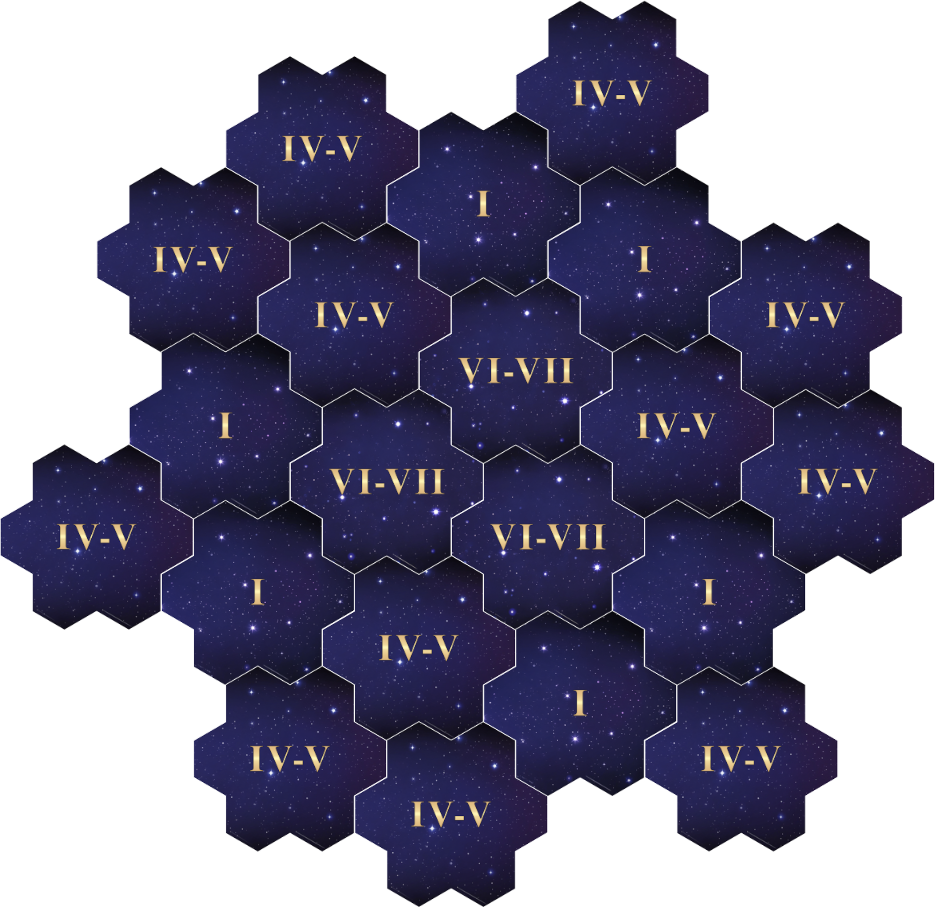
\includegraphics[width=1.0\linewidth]{\maps/shattered_alliance-6p.png}
  \captionof{figure}{\textbf{SCENARIO MAP LAYOUT}}
  \vspace*{\fill}
  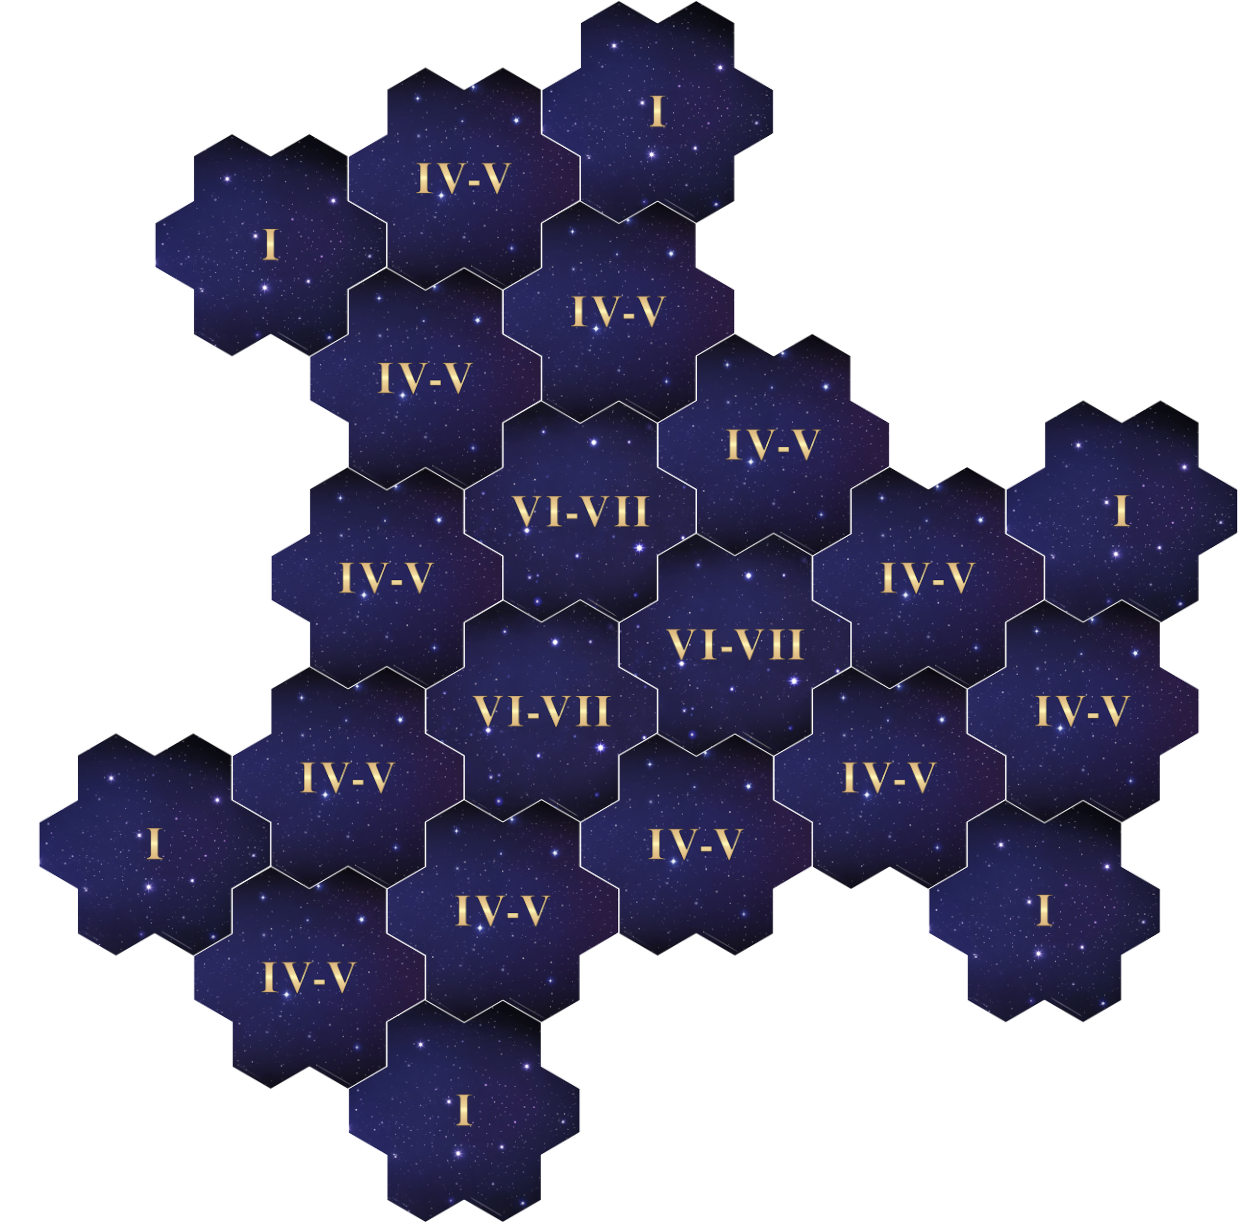
\includegraphics[width=1.1\linewidth]{\maps/shattered_alliance_alt-6p.png}
  \captionof{figure}{\textbf{ALTERNATIVE MAP LAYOUT}}
  \vspace*{\fill}
\end{center}

\vspace*{\fill}

\end{multicols*}
